%%%%%%%%%%%%%%%%%%%%%%%%%%%%%%%
%This is the article LaTeX template for RSC journals
%Copyright The Royal Society of Chemistry 2010
%%%%%%%%%%%%%%%%%%%%%%%%%%%%%%%


\documentclass[8.5pt,twoside,twocolumn]{article}
\oddsidemargin -1.2cm
\evensidemargin -1.2cm
\textwidth 18cm
\headheight 1.0in
\topmargin -3.5cm
\textheight 22cm
\usepackage[super,sort&compress,comma]{natbib} 
\usepackage{mhchem}
\usepackage{times,mathptm}
\usepackage{sectsty}
\usepackage{balance} 
\usepackage{graphicx} %eps figures can be used instead
\usepackage{lastpage}
\usepackage[format=plain,justification=raggedright,singlelinecheck=false,font=small,labelfont=bf,labelsep=space]{caption} 
\usepackage{fancyhdr}
\usepackage{bm}
\usepackage{float}

\pagestyle{fancy}

\newcommand{\update}[1]{{\color{red} #1}}
\newcommand{\e}[1]{\cdot10^{#1}}
\newcommand{\gd}{\dot{\gamma}}

\begin{document}

\thispagestyle{plain}
\fancypagestyle{plain}{
\fancyhead[L]{
\includegraphics[height=8pt]{LH.pdf}}
\fancyhead[C]{\hspace{-1cm}
\includegraphics[height=20pt]{CH.pdf}}
\fancyhead[R]{
\includegraphics[height=10pt]{RH.pdf}\vspace{-0.2cm}}
\renewcommand{\headrulewidth}{1pt}}
\renewcommand{\thefootnote}{\fnsymbol{footnote}}
\renewcommand\footnoterule{\vspace*{1pt}% 
\hrule width 3.4in height 0.4pt \vspace*{5pt}} 
\setcounter{secnumdepth}{5}



\makeatletter 
\def\subsubsection{\@startsection{subsubsection}{3}{10pt}{-1.25ex plus -1ex minus -.1ex}{0ex plus 0ex}{\normalsize\bf}} 
\def\paragraph{\@startsection{paragraph}{4}{10pt}{-1.25ex plus -1ex minus -.1ex}{0ex plus 0ex}{\normalsize\textit}} 
\renewcommand\@biblabel[1]{#1}            
\renewcommand\@makefntext[1]% 
{\noindent\makebox[0pt][r]{\@thefnmark\,}#1}
\makeatother 
\renewcommand{\figurename}{\small{Fig.}~}
\sectionfont{\large}
\subsectionfont{\normalsize} 

\fancyfoot{}
\fancyfoot[LO,RE]{\vspace{-7pt}
\includegraphics[height=9pt]{LF.pdf}}
\fancyfoot[CO]{\vspace{-7.2pt}\hspace{12.2cm}
\includegraphics{RF.pdf}}
\fancyfoot[CE]{\vspace{-7.5pt}\hspace{-13.5cm}
\includegraphics{RF.pdf}}
\fancyfoot[RO]{\footnotesize{\sffamily{1--\pageref{LastPage} ~\textbar  \hspace{2pt}\thepage}}}
\fancyfoot[LE]{\footnotesize{\sffamily{\thepage~\textbar\hspace{3.45cm} 1--\pageref{LastPage}}}}
\fancyhead{}
\renewcommand{\headrulewidth}{1pt} 
\renewcommand{\footrulewidth}{1pt}
\setlength{\arrayrulewidth}{1pt}
\setlength{\columnsep}{6.5mm}
\setlength\bibsep{1pt}

\twocolumn[
  \begin{@twocolumnfalse}
\noindent\LARGE{\textbf{Nonlinear Rheology of Layered Smectic Liquid Crystals}}
\vspace{0.6cm}

\noindent\large{\textbf{O. Henrich\textit{$^{a}$}, D. Marenduzzo\textit{$^{b}$}, K. Stratford\textit{$^{c}$} and M.E. Cates \textit{$^{b}$}}
}\vspace{0.5cm}
%Please note that \ast indicates the corresponding author(s) but no footnote text is required. 


\noindent\textit{\small{\textbf{Received Xth XXXXXXXXXX 20XX, Accepted Xth XXXXXXXXX 20XX\newline
First published on the web Xth XXXXXXXXXX 200X}}}

\noindent \textbf{\small{DOI: 10.1039/b000000x}}
\vspace{0.6cm}
%Please do not change this text.

\noindent \normalsize{In this work we present large scale computer simulations of the bulk rheology of a smectic liquid crystal at intermediate to large values of the shear flow, threfore in the nonlinear regime. In two dimensions we find that, according to the thermodynamic parameters, shear may either align the system and stabilise an almost regular lamellar phase, or induce the nucleation and proliferation of defects in the smectic layers. In this last case, defects may be progressively annealed by slowly decreasing the applied shear rate, so that there are marked memory effects and the rheology is history-dependent. Finally, selected simulations in three dimensions show shear-induced ordering rather than defect nucleation, thus pointing out to a dramatic effect of dimensionality on the physics of the system.}
\vspace{0.5cm}
 \end{@twocolumnfalse}
  ]

%Footnotes
%Please use \dag to cite the ESI in the main text of the article.
%If you article does not have ESI please remove the the \dag symbol from the title and the above footnotetext.

\footnotetext{\textit{$^{a}$~University College of London, London, UK}}
\footnotetext{\textit{$^{b}$~SUPA, School of Physics and Astronomy, University of Edinburgh, JCMB Kings Buildings, Mayfield Road, Edinburgh, EH9 3JZ, Scotland.}}
\footnotetext{\textit{$^{c}$~EPCC, School of Physics and Astronomy, University of Edinburgh, JCMB Kings Buildings, Mayfield Road, Edinburgh, EH9 3JZ, Scotland.}}

%additional addresses can be cited as above using the lower-case letters, c, d, e... If all authors are from the same address, no letter is required

%\footnotetext{\ddag~Additional footnotes to the title and authors can be included \emph{e.g.}\ `Present address:' or `These authors contributed equally to this work' as above using the symbols: \ddag, \textsection, and \P. Please place the appropriate symbol next to the author's name and include a \texttt{\textbackslash footnotetext} entry in the the correct place in the list.}


\section{Introduction}
Instances of soft complex fluids surrounding us abound: for instance paint, cosmetics and food products such as ketchup, mayonnaise, yogurth etc are all well-known examples of colloidal suspensions, where particles or droplets are suspended in a viscous fluid. Biological systems also include a large range of soft materials: for instance the intracellular network of actin fibers constituting the cytoskeleton of mammalian cells is a polymeric fluid, as is the DNA making up the bacterial nucleoid or eukaryotic chromosomes, or the viral genome of bacteriophages, where enhanced confinement imparts strong liquid crystalline character. Soft materials such as liquid crystalline fluids, with or without colloidal inclusions, are also of importance technologically, for instance when they are used to build up display devices or in biosensing.

Rheology gives a powerful way to characterise macroscopic physical properties of a soft material such as its viscosity, elastic and loss moduli, which quantify, for instance, its rigidity, response to applied forces or stresses etc. While in a Newtonian, viscous fluid, shearing gives rise to a stress which is linearly proportional to the applied shear rate -- the slope being the viscosity -- in complex fluids flow is often non-Newtonian and such a simple linear relation no longer holds. Thus, viscoelastic complex fluids may be shear thickening or shear thinning, if their effective viscosity increases or decreases with applied shear. They may even spontaneously phase separate when flowing, giving rise to shear bands which are familiar in the rheology of liquid crystals in the vicinity of the isotropic-nematic transition, and in wormlike micelles.

The rheological properties of a non-Newtonian fluid are often linked to the microstrucure of the material. For instance, in the flow of polydomain liquid crystals, which are not uniformly ordered, the existence of regions with conflicting director patterns leads to a non-linear relation between shear stress and applied shear rate. Another intriguing example of strongly non-Newtonian rheology is region I flow in polymeric nematic liquid crystals. While our understanding of the physics of region I flow is far from complete, it is thought that a defect network may form and lead to much enhanced viscosity, with marked shear thinning, $\eta \sim \dot{\gamma}^{\alpha}$, and an exponent $\alpha$ typically between 0 and 1. Particularly relevant to our current work is the rheology of layered systems, such as smectics and cholesterics. Experiments involving any of such soft materials typically lead to vastly different results, according to whether the system has been ordered prior to the rheological study, for instance via preshearing, or not. In the latter case the measured viscosities are much larger, and just as in polydomain or region I nematic flow, this stiffening is usually associated to the presence of defects in the sample. An intriguing flow mode which is possible in layered system is permeation, through which the individual molecules in the fluid displace keeping the defect pattern intact in steady state. This leads to increased dissipation and hence to a larger viscosity. A well-known example of permeation flow is the one which occurs e.g. in cholesterics which are sheared or pushed along the direction of the cholesteric helix. However, one would expect permeation flows to be possible also when a non-translationally invariant defect pattern is present in the system, so that it may occur to some extent also in quenched smectics for instance.
Lamellar rheology is also of interest for a number of additional intriguing phenomenological observations beyond their nonlinear shear-stress curve. For instance, in block-copolymers one may observe, under some conditions, shear-induced phase transitions from the microphase separated state to ordered phases like the lamellar one~\cite{Cates89,Koppi93,Fredrickson94}, and it would be desirable to extend our theoretical understanding of such switches. Furthermore, lyotropic layered liquid crystals have sometimes been observed to form an onion phase \cite{Panizza96,Iwashita07} which can happen either spontaneously \cite{Gomati87,Boltenhagen92,Fournier94,Ramos04} or under shear \cite{Diat93} -- the mechanism underlying such pattern formation has remained elusive to date. 


Despite the wealth of experimentally available results, and the importance of rheology to for instance industrial applications, flow behaviour remains challenging to study theoretically. This is mainly in view of the highly non-linear equations of motion which require either drastic approximations or challenging computer simulations. At the same time, realistic modelling eventually requires the simulation of a fully 3-dimensional flow, which is particularly expensive computationally. In this work, we aim to contribute to fill in the gap towards realistic large scale computational studies of complex fluids, and our focus is the physics of smectics under shear. For another example of large scale simulations for complex fluids, see Ref.~\cite{Saksena09} where sheared gyroid phases were simulated.
We shall concentrate here on intermediate values of the shear rate for which, as we shall see, we may observe either an approximately linear or markedly non-linear behaviour of the system, according to the thermodynamic parameters. In our treatment, we describe smectics via a Brazovskii free energy functional \cite{Brazovskii75}, which provides a robust framework to study systems like miscelles, surfactants, smectic liquid crystals and block-copolymer.

%Copolymer consist of type-A polymers covalently bonded to type-B polymers and can self-organize in a variety of phases, ranging from spherical phases over hexagonal cylindrical phases to lamellar phases or bicontinuous gyroid phases \cite{Bates90}. 

The governing equations in our model are a convection-diffusion equation for the scalar order parameter, which represents the density difference of the two phases and the Navier-Stokes equation with a stress tensor that contains extra contributions due to the presence of the lamellar interfaces.
In our approach the dynamical equations are solved using a combination of finite difference scheme for the convection-diffusion equation and the lattice Boltzmann method (LBM) \cite{Succi} for the Navier-Stokes equation.
The LBM solves the Boltzmann equation on a regular lattice for a representative fluid that obey simplified dynamics in terms of a free propagation step of quasi-particles followed by a collision step, in which the particles interact.
The LBM solves the Navier-Stokes equation in the limit of small Mach numbers $Ma\ll1$ and has been largely applied to fluid flow in complex geometries, where it is superior to conventional methods of computational fluid dynamics.

Our main finding is that as anticipated above depending on system parameters we find that a smectic phase may lead to vastly different rheological responses. 
When thermodynamic forces are weaker with respect to viscous, flow-induced, ones, shear quickly orders the system into a lamellar phase, with only a few defects. The rheology in this regime is Newtonian, and the shear stress is linear in the applied shear rate. If, on the other hand, thermodynamic forces are larger, we observe that shear actually leads to the nucleation of new defects, and the rheology is highly nonlinear, with the shear rate proportional to $\dot{\gamma}^{\alpha}$, with $\alpha\simeq 0.87$, leading to a shear thinning behaviour. Such a behaviour is qualitatively reminiscent of the one found experimentally in XXX, where the numerical value of $\alpha$ was however different. In this regime we also find that the rheology is history dependent, as the defect density decreases for instance if the shear rate is ramped down gradually. Finally, intriguingly, dimensionality appears to play a key role: within our 3D simulations, we have indeed not been able to enter the nonlinear rheology regime with defect nucleation, and we always observe a shear-induced ordering into a lamellar phase. More research and parameter steering will be needed to make this observation more quantitative.
We note that sheared smectics have been studied extensively via simulations in the literature~\cite{Swift96,Gonnella97,Gonnella98,Xu03,Xu05,Xu06a,Xu06b}, but because of computational constraints almost all results were limited to two dimensions and smaller strains than the ones considered here. Furthermore in this work we use Lees-Edwards boundary conditions which allow us to probe the true bulk rheology of the system, at variance with previous work which employed solid walls and different boundary conditions, which introduce finite size and boundary effects into the physics.
 
This paper is organised as follows. In Sec.II we introduce the model, including its equilibrium properties, the full stress tensor and the dynamical equations.
We briefly sketch how we derive structural information from the order parameter and describe our defect quantification procedure, which measures the local alignment of the lamellar structure.
We present results of the two dimensional case in In Sec.III, discuss the morphology, average and local shear stress densities and first normal stress differences and their relation to the defect structure.
We also show structure factors for various flow states and flow curves.
In Sec. IV we compare our 2D-results with results in three dimensions. 
A summary with conclusions closes the paper in Sec.V.

\section{Model and Definitions}

The equilibrium phase is found for an order parameter field $\phi({\bm r})\equiv \phi$ that minimizes the Landau-Brazovskii free energy functional \cite{Brazovskii75,deGennes}.
\begin{eqnarray}
{\cal F}[\phi]&=&\int d^dx f(\phi({\bm x}))\nonumber\\
&=&\int d^dx\left\{\frac{a}{2}\phi^2+\frac{b}{4}\phi^4+\frac{\kappa}{2} ({\bm \nabla}\phi)^2+\frac{c}{2}(\nabla^2\phi)^2\right\}\label{FE-functional}
\end{eqnarray}
The parameters $b$ and $c$ are positive to ensure stability. 
For $a>0$ there is only one solution $\phi\equiv0$ which minimizes the functional and corresponds to the disordered state.
For $a<0$ a microphase separation occurs and depending on the sign of $\kappa$ either two homogenous phases coexist ($\kappa>0$) or a transition to an ordered lamellar phase state takes place ($\kappa<0$) because the formation of interfaces become energetically favourable.\\
The dynamics of the binary fluid is governed by a convection-diffusion equation with a diffusive current proportional to the chemical potential $\mu$, which is the functional derivative of ${\cal F}$ with respect to $\phi$.
\begin{equation}\label{OPEOM}
\partial_t \phi +{\bm \nabla}({\bm u}\phi) = M \nabla^2 \frac{\delta \cal F}{\delta \phi}=M \nabla^2 \mu 
\end{equation}
The coefficient $M$ herein plays the role of a mobility coefficient.\\
If the fluid is incompressible, the evolution of the velocity ${\bm u}$ obeys a Navier-Stokes equation
\begin{equation}\label{NSE}
\partial_t u_\alpha + (u_\beta \nabla_\beta) u_\alpha = \partial_\beta \sigma_{\alpha \beta}. 
\end{equation}
The stress tensor reads
\begin{equation}
\sigma_{\alpha \beta}=-P^{th}_{\alpha \beta} +\eta (\partial_\alpha u_\beta + \partial_\beta u_\alpha).
\end{equation}
It consists of a hydrodynamic part, which is proportonial to the viscosity $\eta$ of the solvent and a thermodynamical part $P^{th}$ that depends on the order parameter.
The latter can be calculated from the free energy functional:
\begin{equation}
P_{\alpha\beta}^{th}=\left(\phi\frac{\delta {\cal F}}{\delta \phi} -f(\phi)\right) \delta_{\alpha\beta} + D_{\alpha \beta}(\phi).
\end{equation}  
In this expression the symmetric tensor $D_{\alpha\beta})$ has been added to make the pressure tensor divergence free and to guarantee the mechanical equilibrium \cite{Evans79}.
The thermodynamic pressure tensor is given by
\begin{equation}
P^{th}_{\alpha \beta}=p\, \delta_{\alpha \beta} + P^{chem}_{\alpha \beta}
\end{equation}
with an isotropic pressure contribution
\begin{eqnarray}
p&=& \frac{a}{2}\phi^2+\frac{3b}{4}\phi^4-\kappa\left(\phi(\nabla^2\phi)+\frac{1}{2}({\bm \nabla}\phi)^2\right)\nonumber\\
& &\quad+c\left(\phi(\nabla^2)^2\phi+\frac{1}{2}(\nabla^2\phi)^2+\partial_{\gamma}\phi\partial_\gamma(\nabla^2\phi)\right)
\end{eqnarray}
and an anisotropic part
\begin{equation}
P^{chem}_{\alpha \beta}=\kappa\partial_\alpha\phi\partial_\beta\phi -c \left(\partial_\alpha\phi\partial_\beta(\nabla^2\phi)+\partial_\beta\phi\partial_\alpha(\nabla^2\phi)\right).
\end{equation}

The Navier-Stokes Eq.\ref{NSE} was solved at every timestep by means of a multi-relaxation time lattice-Boltzmann solver \cite{dHumieres02,Adhikari05} using the D3Q19 model.
The velocity field were then put into the convection-diffusion equation Eq.\ref{OPEOM} and solved at the same timestep. 
We assumed periodic boundary conditions along the flow and vorticity direction and Lees-Edwards boundary conditions (BC) \cite{Wagner02} along the direction of the velocity gradient.
The total number of Lees-Edwards planes was varied according to the size of the simulation so that the distance of two planes was always 16 lattice sites.
To impose simple shear flow, the planes in the upper half of the velocity gradient direction were moved at a constant speed in positive flow direction, whereas the planes in the lower hemisphere were moved in negative flow direction.\\
Structural information in Fourier space was obtained from the static structure factor $C({\mathbf k})$, defined as
\begin{equation}
C({\mathbf k})=\phi({\mathbf k})\phi(-{\mathbf k}),
\end{equation}
with $\phi({\mathbf k})$ as normalised Fourier-transform of the order parameter.
The transform itself was calculated using the FFTW-library \cite{FFTW}.\\
In order to analyse the relation between rheological quantities and the morphology of the system it was necessary to quantify the number of defects.
For this purpose we defined an alignment factor $X_i$, which measures the average projection of the normalised order parameter gradients onto the gradient at site $i$.
More explicitely the alignment factor $X_i$ is given as
\begin{equation}\label{alignment}
X_i=\frac{1}{N_{nn}} \sum_{j=1,N_{nn}}\left(\frac{\nabla \phi_i \cdot \nabla \phi_j}{|\nabla\phi_i||\nabla\phi_j|}\right)^2. 
\end{equation}
$N_{nn}$ is the number of nearest neighbours ($N_{nn}=8$ in 2D and $N_{nn}=26$ in 3D).
For smooth alignment and small curvature of the lamellae $X_i$ is very close to unity.
At the endpoints of the lamellae or in regions where their orientation changes abruptly it departs form unity and takes up smaller positive values.
By setting a threshold $\xi$ it is possible to detect domains where the order parameter structure deviates from what would be recognised by the eye as an aligned configuration.
We found a threshold of $\xi=0.8$ to work quite well for our requirements.
Unfortunately this defect detecting protocol is not able to assign only a single defect site to a disturbed region in the order parameter structure as normally more than one site close to a defect would have an alignment factor below the threshold.
However, as the number of sites per defect is roughly constant throughout the sample, it is still useful for quantifying the degree of alignment and comparing different systems or flow conditions.\\
By relating the number of defects sites with $X_i$ below the threshold to the total number of sites it is possible to define a defect density:
\begin{equation}\label{defectdensity}
\rho_D=\frac{1}{N} \sum_{i=1,N} \theta(\xi-X_i).  
\end{equation}
The function $\theta$ is the Heaviside function and $N=N_x\times N_y \times N_z$ the total number of sites in the simulation.
The exact value of the defect density depends clearly on the lamellar width and of course on the threshold $\xi$ for the alignment parameter.

\subsection*{Parameter Mapping to Physical Units}

In the following we describe how the simulation units can be mapped onto real physical units.
It is necessary to calibrate the scales for mass density, length and time or alternatively as we do for mass density, length and energy density.\\
As usual we set the lattice spacing $l$, time step $\Delta t$ and mass density of the reference fluid $\rho_0$ all to unity in LB units (LBU).
It is straightforward to determine the unit of mass. 
A typical block copolymers or liquid crystal has a mass density the region of $10^3 {\rm kg m}^{-3}$, which is of the order ${\cal O}(1)$ in LBU.
Hence $1 {\rm kg m}^{-3}=10^{-3}$ LBU.\\
In order to get a length scale we compare the average distance of two lamellae in Fig.\ref{fig12} with characteristic values of diblock copolymers in the lamellar phase or smectic liquid crystals.
Typical values for the lamellar width are roughly 50nm, which make about 10 LBU in our simulation.
Therefore the unit length $l$ in LBU corresponds to about 5nm in physical space.\\
The energy scale is slightly more difficult to calibrate.
We use the fact that both diblock copolymer melts and smectic liquid crystals belong to the Brazovskii class.
This has been already pointed out by Leibler \cite{Leibler80} in his seminal work on microphase separation in block copolymers.
The Landau free energy functional we are using can be transformed into a Brazovskii-type of form and coefficients can be compared \cite{Xu05, Fredrickson89}.
The energy density scale in our functional \ref{FE-functional} is set by the coefficients $-a=b$ of the quadratic and quartic term, respectively.
Referring to \cite{Fredrickson89} we can derive an expression that relates $b$ to Leibler's original parameters.
This formula reads 
\begin{equation}
b=\frac{u_0 k_B T}{6}=\frac{c^4\lambda k_B T}{6} \rho_c,
\end{equation}
whereas $\rho_c$ is the number density of chains per unit volume,
often expressed as $\rho_c=\sqrt{N/6^3} R_g^{-3}$ with $N$ as roughly the number of Kuhn segments and $R_g$ as radius of gyration.
Typical values are $N\simeq10^4$ and $R_g\simeq 100{\rm nm}$.
With $c=1.1019$ and $\lambda=106.18$ taken from the same reference and assuming $k_B T\simeq 4\e{-21} {\rm J}$ at room temperature, we get an estimate for $b$ of roughly $5\e{2} {\rm J m}^{-3}$, which is $b=5\e{-4}$ in LBU.
Hence the LB unit of energy density is about $1\e{6} \rm{Pa}$.\\
We can now combine the scales for energy density, length and mass density to get an estimate for the time scale.
As ${\rm s}^2=\rm{kg}\, \rm{m}^{-3}\, \rm{Pa}^{-1}\rm{m}^2=1\e{-3+6+14} \rm{LBU}\simeq1\e{17} \,{\rm LBU}$, we derive that $1 \rm{s}\simeq3\e{8}$LBU and one LB timestep $\Delta t$ corresponds to roughly 3ns.\\
Finally we want to get an estimated scale for shear rates. 
A common way to quantify them is the dimensionless Peclet number, which measures the transport of a particle as the ratio of the rate of advection to the rate of diffusion.
The Peclet number can be defined as $Pe_0=\gd\, D^2/D_0$, where $\gd$ is the rate of strain, $D$ is a characteristic length, e.g. the diameter of a particle and $D_0$ is the diffusivity.
The highest shear rate we apply is $2\e{-4}$ in LBU, basically reciprocal LB time units.
With the above value for $\Delta t$ we can convert this into about $5\e{4}{\rm s}^{-1}$.
If we suppose the Stokes-Einstein diffusion constant is a good approximation for $D_0$, we get for an object of the size of $D\simeq5\e{-8}$ at room temperature in a low viscous solevent like water values of about $D_0=1\e{-11} \rm{m}^2\rm{s}^{-1}$.
This results in Peclet number of the order ${\cal O}(10)$ and means shear rates $\gd={\cal O}(10^{-4})$ in LBU correspond to a Peclet numbers $Pe_0={\cal O}(10)$.

\section{Results}

Our discussion will be in two parts, beginning with simulations in two dimensions for a system A and a slightly softer system B of size $N_x\times N_y=1024\times 512$ and $N_x \times N_y=512\times 256$ respectively for longtime runs.
The stiffness of the system was controlled by modifying the Landau parameters $a$ and $b$ of the bulk terms in the free energy functional \ref{FE-functional} with the parameters $\kappa$ and $c$ multiplying the gradient terms held constant.
By this we obtained slightly different segregation levels in both systems A and B, whereas the lamellar distance was virtually the same.\\
The second part of our discussion consits of simulations in three dimensions using identical parameters to system A and a box size $N_x\times N_y\times N_z=128\times256\times128$.
We will refer to this system as system C.
Table \ref{tab1} at the end of this paragraph provides an overview of all simulation parameters.


\subsection*{Results in Two Dimensions}
There is some freedom regarding the parametrizaton of binary fluids using the Landau-Brazovskii free energy approach \ref{FE-functional}.
Hence we stuck in the present work to parameters, which have been found to cover the relevant morphology of lamellar systems and produce stable outcomes in previous studies \cite{Kendon01,Xu03, Xu06b}. 
We performed simulations for a variety of parameter sets with Landau parameters $1\cdot10^{-3}\le-a=b\le5\cdot10^{-5}$ and viscosities $8.33\cdot10^{-4}\le\eta\le 0.833$.
Reasonable numerical stability was attained for all Landau parameters in this range and for viscosities $\eta\ge 8.33\e{-3}$.
The morphology of the lamellar structure and the kinetics of the spinodal decomposition depended on the specific choice though.
Smaller Landau parameters slowed down the ripening speed of the lamellar structure, which is consistent with the fact that the system is closer to the critical point where the phase microphase separation occurs.
Higher viscosities led to shorter interfaces, whereas values around the lower threshold invoked longer interfaces.
\begin{figure}[!]
\centering
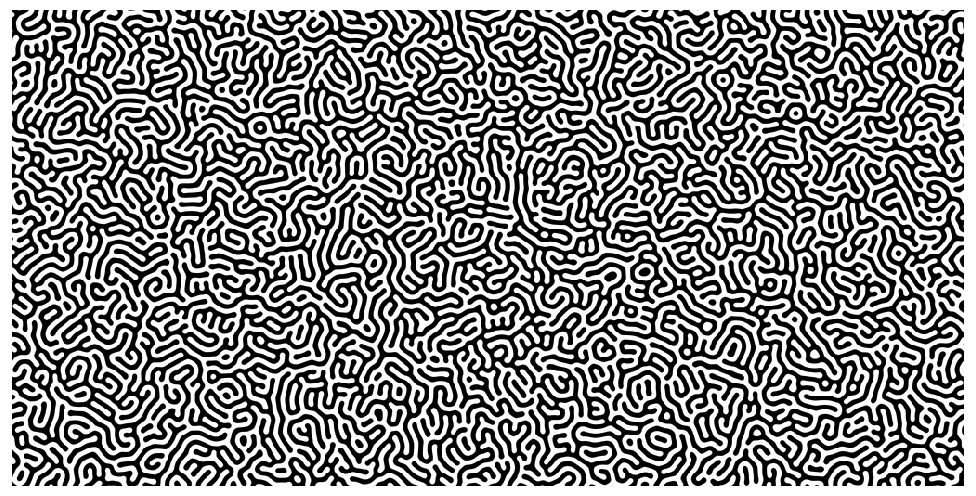
\includegraphics[angle=0,width=0.5\textwidth]{phi_run703_320.jpg}\\
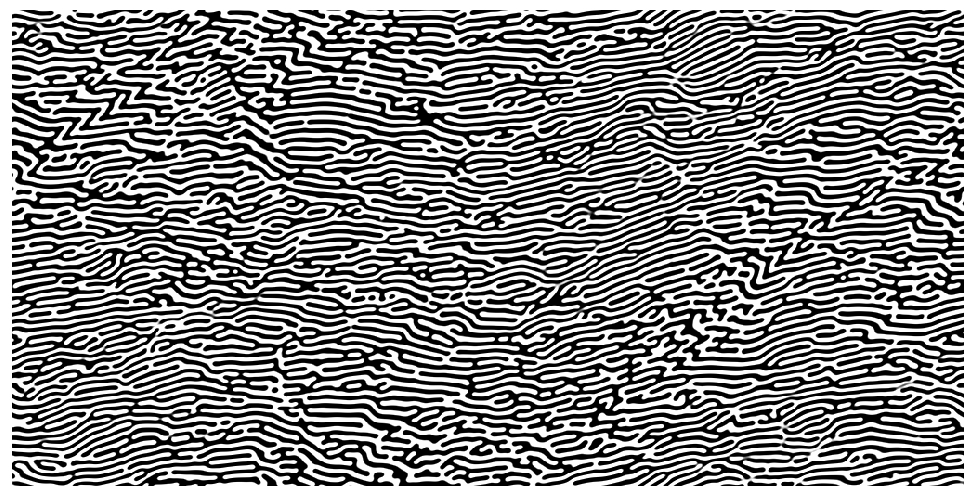
\includegraphics[angle=0,width=0.5\textwidth]{phi_run704_500.jpg}\\
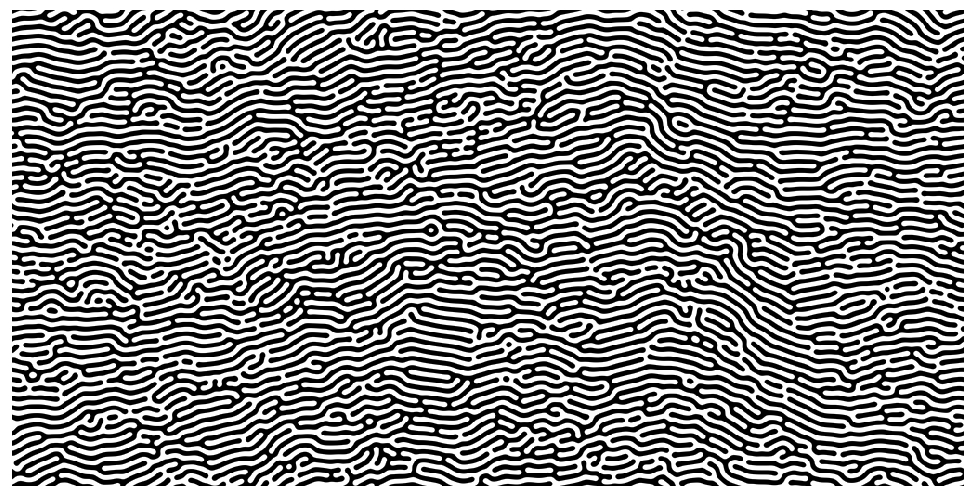
\includegraphics[angle=0,width=0.5\textwidth]{phi_run705_1280.jpg}
\caption{Order parameter $\phi$ of system A: after equilibration (timestep $t=3.2\e{5}$, top), at $\dot{\gamma}=1\cdot10^{-4}$ ($t=5\e{5}$, centre) and after switch-off ($t=1.28\e{6}$, bottom). Gray scaling from black to white corresponds to values of $-1\le\phi\le1$}
\label{fig1}
\end{figure}
This effect has been reported before \cite{Gonnella97} and was more pronounced for softer systems with smaller Landau parameters, although not quite to the same extent as in the above reference.
Under shear higher viscosities caused the lamellae to be much less homogenous in shape and thickness.\\
In the following we will show characteristic results for viscosity $\eta=8.33\e{-2}$ and the stiffer system A with $-a=b=5\e{-4}$ and the softer system B with $-a=b=5\e{-5}$, respectively.\\
The top picture in Fig. \ref{fig1} shows the order parameter $\phi$ at the end of the equilibration phase prior to shearing.
The equilibrium structure is completely isotropic and exhibits a lamellar spacing of roughly 10 lattice sites.
If shear flow is imposed, the lamellae start to align with the flow.
\begin{figure}[!]
\centering
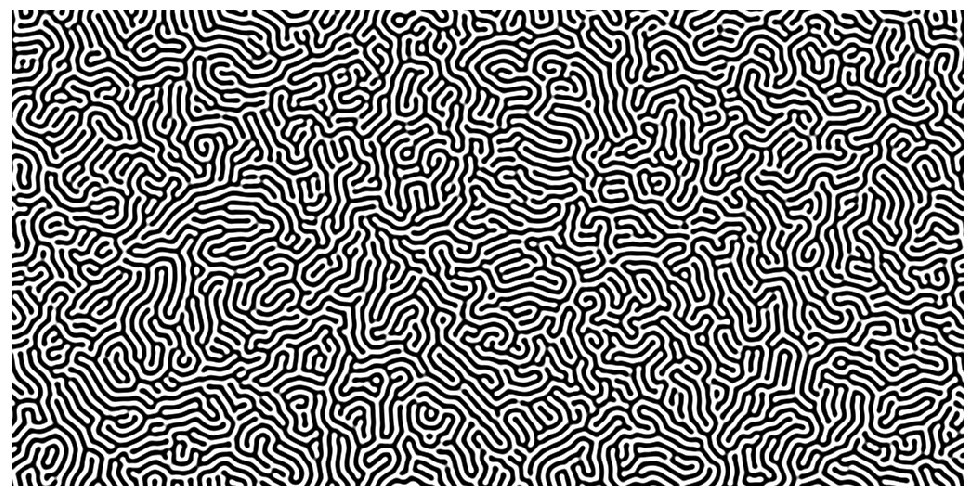
\includegraphics[angle=0,width=0.5\textwidth]{phi_run707_320.jpg}\\
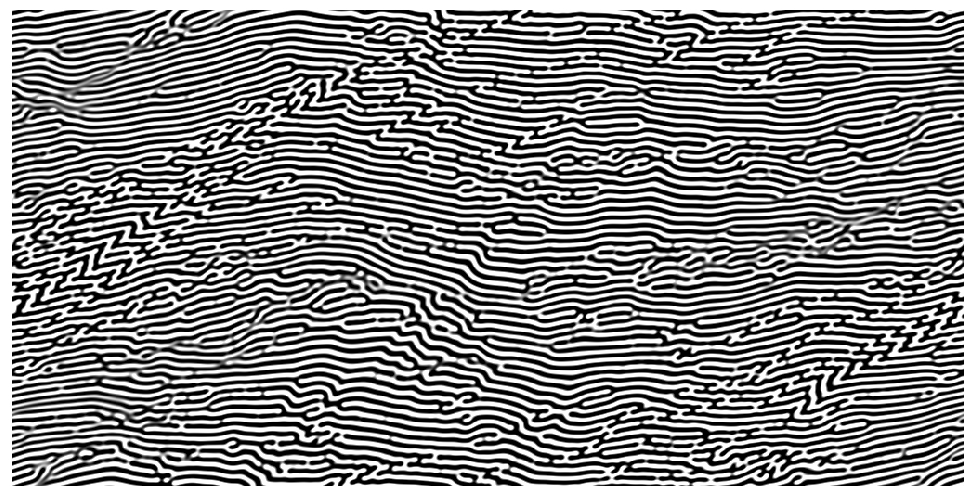
\includegraphics[angle=0,width=0.5\textwidth]{phi_run710_800.jpg}\\
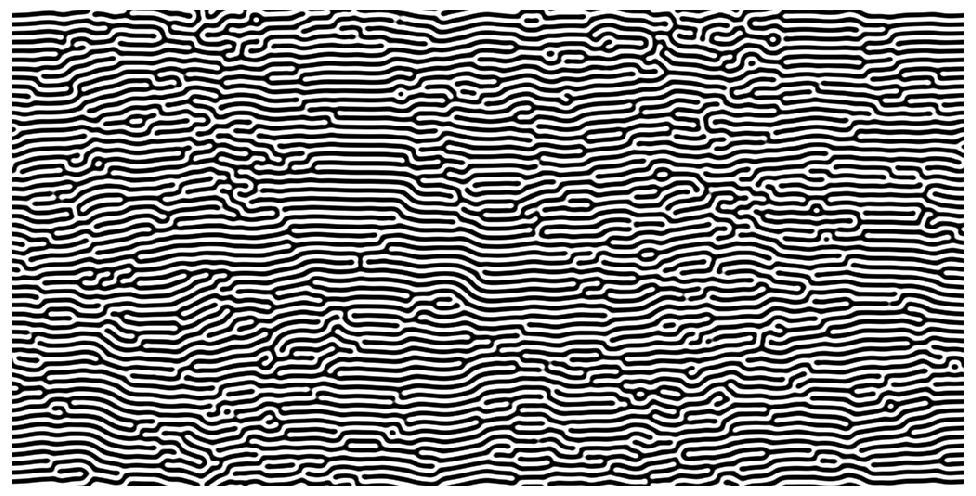
\includegraphics[angle=0,width=0.5\textwidth]{phi_run765_1280.jpg}
\caption{Order parameter $\phi$ of system B: after equilibration (timestep $t=3.2\e{5}$, top), at $\dot{\gamma}=1\cdot10^{-4}$ ($t=8\e{5}$, centre) and after switch-off ($t=1.28\e{6}$, bottom)}
\label{fig2}
\end{figure}
In this paragraph the flow direction and the direction of the velocity gradient are x and y, respectively.
The apparent flow due to the effect of the Lees-Edwards planes is always in positive x-direction in the upper half and in negative x-direction in the lower half of the box.
After a short startup phase in which the order parameter remains rather homogenous, regions of reduced and increased lamellar width emarge and the spacing deviates from its equilibrium value.
These regions are advected with the flow while they undergo an affine stretching.
The centre picture in Fig. \ref{fig1} shows an example at an intermediate time step at shear rate $1\e{-4}$.
In a previous work on binary fluids and lamellar systems in shear flow \cite{Xu06b} another shear-induced structure was found.
However, the reported results differ from our observations in the following aspects.
First of all, the shear-induced structures emerge at the centre and remain located, while ours occur in bandlike patterns that are wrapped around the periodic boundaries.
Moreover those bear the characteristics of a shear banding region exhibiting a reduced local shear rate.
These differences may be a direct consequence of the different boundary conditions.
While we applied Lees-Edwards BC along y and periodic boundary conditions along x for all quantities, \cite{Xu06b} seem to have used sort of hybrid scheme.
\begin{figure}[!]
\centering
\hspace*{-0.1cm}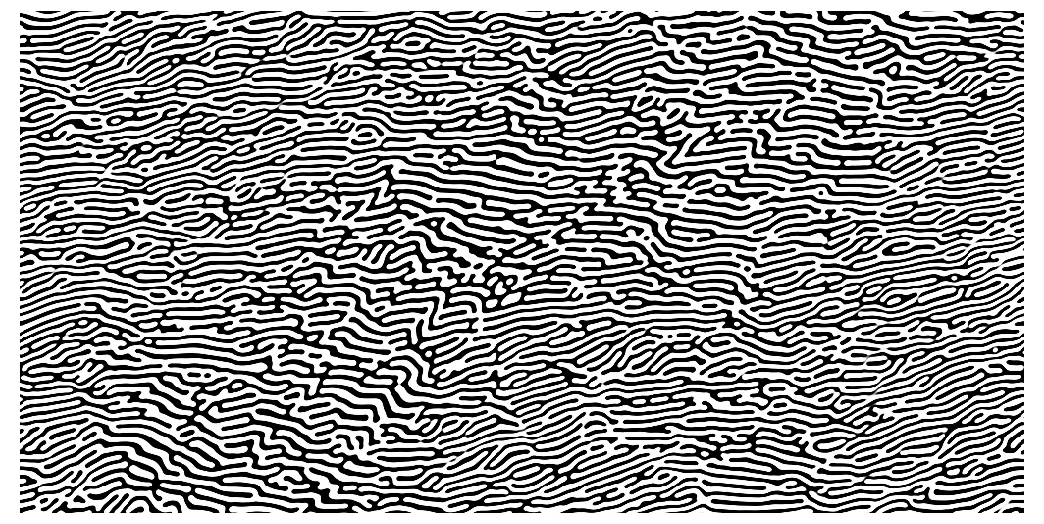
\includegraphics[angle=0,width=0.5\textwidth]{phi_run704_400.jpg}
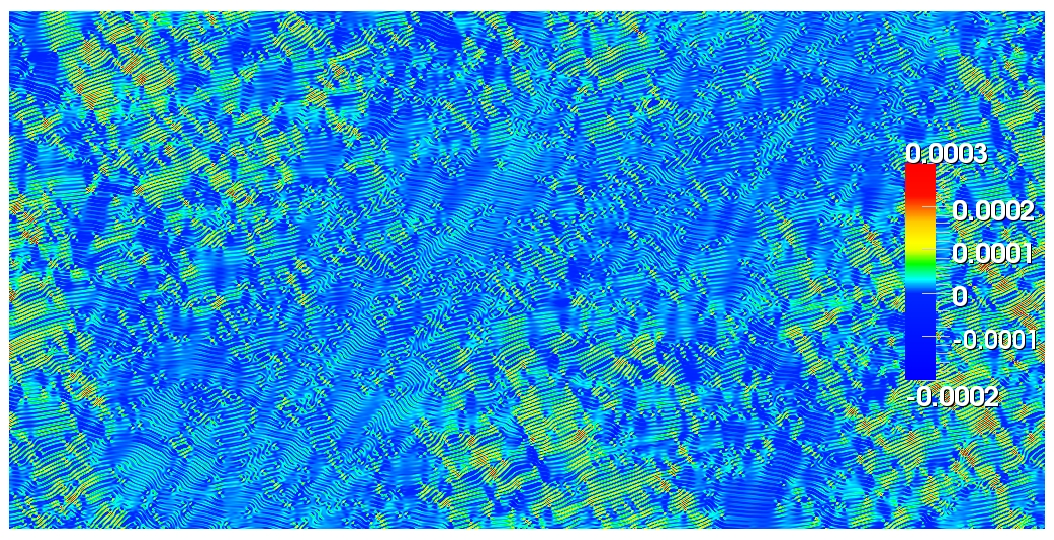
\includegraphics[angle=0,width=0.49\textwidth]{shear_str_run704_400.jpg}
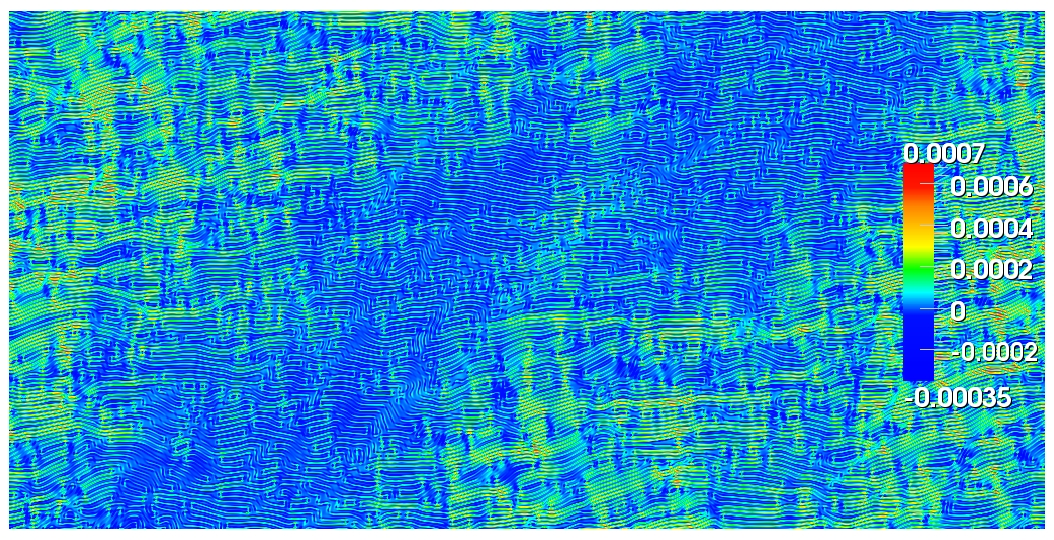
\includegraphics[angle=0,width=0.49\textwidth]{N1_run704_400.jpg}
\caption{Order parameter $\phi({\mathbf r})$ (top), shear stress $\sigma_{xy}({\mathbf r})$ (centre) and first normal stress differences $N_1({\mathbf r})$ (bottom) of system A at $t=4\e{5}$}
\label{fig3}
\end{figure}
\begin{figure*}[!]
\centering
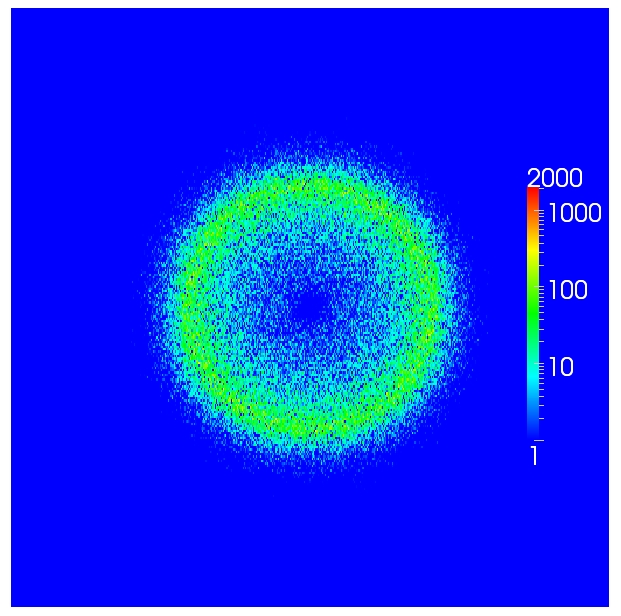
\includegraphics[angle=0,width=0.33\textwidth]{ck_run703_320.jpg}
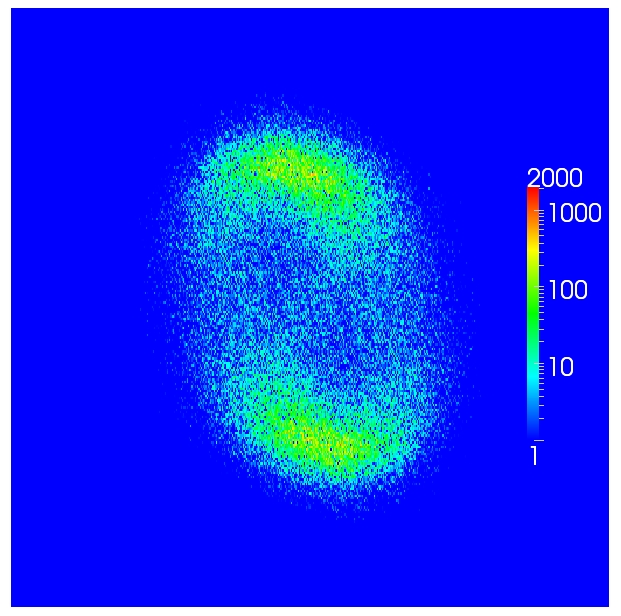
\includegraphics[angle=0,width=0.33\textwidth]{ck_run704_500.jpg}
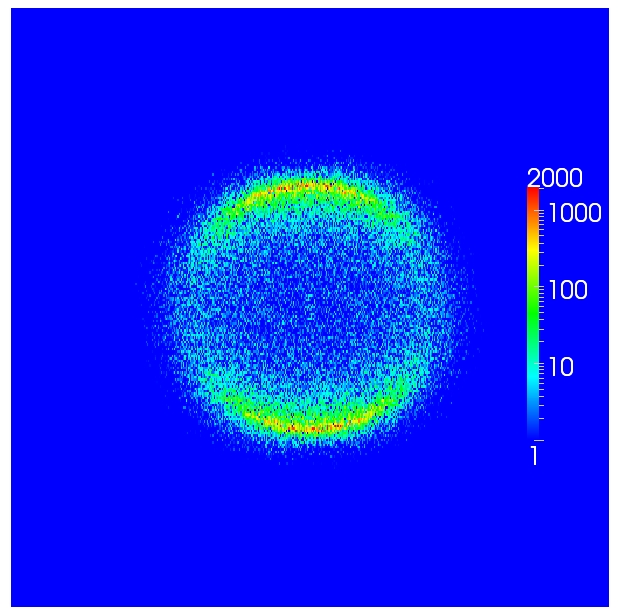
\includegraphics[angle=0,width=0.33\textwidth]{ck_run705_1280.jpg}
\caption{Structure factor $C({\bm k})$ of system A: Shown are states after equilibration at $t=3.2\e{5}$ (left), at $\dot{\gamma}=1\cdot10^{-4}$ and $t=5\e{5}$ (centre) and after switch-off at $t=1.28\e{6}$ (right). The sections shown correspond to wavevectors on the interval $k_x, k_y \in [-\pi/2 l,\pi/2 l]$.}
\label{fig4}
\end{figure*}
To our understanding they applied Lees-Edwards BC for the order parameter only, but placed solid moving walls at the upper and lower boundaries in the lattice Boltzmann part.
Identical to our setup periodic BC in flow direction were applied for both order parameter and momentum flux.
The it might be that \cite{Xu06b} have not simulated bulk flow behaviour but rather flow in a confined geometry and the shear-induced structure they observe might be a consequence of this difference.\\ 
After switching off of the shear flow the expanded regions contract and the compressed regions expand and the system returns to a state with homogenous lamellar width, seemingly close to the equilibrium value.
The final state for which the relaxation has virtually come to a standstill is shown in the bottom picture of Fig. \ref{fig1}. 
The lamellar interfaces remain more or less oriented, but due to the expansion and contraction of the lamellae some individual domains show large angles with the previous flow direction. 
The length of the interfaces varies considerably, which is appears to be another residue of the inhomogeneities in the flowing state.\\
Fig. \ref{fig2} shows equivalent states for the softer system B.
The characteristic results of Fig. \ref{fig1} are retained, but the interfaces in all states tend to be longer.
The lamellar alignment in flow direction after switch off is more pronounced.\\ 
Fig. \ref{fig3} relates the inhomogeneities in the morphology to rheological quantities.
The pictures show the order parameter $\phi$, shear stress density $\sigma_{xy}({\bm r})$ and first normal stress difference density $N1({\bm r})=\sigma_{xx}({\bm r})-\sigma_{yy}({\bm r})$ of system A in steady shear flow at shear rate $\dot{\gamma}=1\e{-4}$.
Where the system is extendend and the lamellar width is larger compared to the equilibrium state, both shear stress and first normal stress differences have low positive or negative values.
Large positive values occur in the regions where the lamellae are squeezed.
The peak values in lattice units are in the region of $-2\e{-4}$ and $3\e{-4}$ for the shear stress and  $-3.5\e{-4}$ and $7\e{-4}$ for the normal stress differences.
Despite the local negativity of quantities, the overall average are still positive for all times.
Very similar results with smaller peak magnitudes are obtained for system B, which appears somewhat more homogenous.\\
Fig. \ref{fig4} shows structure factors $C({\bm k})$ for the three states depicted in Fig. \ref{fig1}.
At first isotropic after the microphase separation and equilibration, $C({\bm k})$ has a distinct peak at $|{\bm k}|\simeq \pm0.2\pi/l$.
In steady shear flow the structure factor develops two distinct though rather broad peaks, which are situated at $k_x\simeq\mp 0.012\pi/l, k_y\simeq\pm 0.22 \pi/l$.
It is interesting to see that the Fourier-vector of the peak position pics up a small component in x-direction, indicating on average a slight tilt of the structure.
The tilting orients the lamellae away from the direction of flow and towards the velocity gradient direction, which is the direction of extension in simple shear flow.
The position of the peak is almost constant throughout the entire simulation.
The average lamellar distance decreases from about 10 lattice sites in the quiescent state to about 8.5 lattice sites.
However, after switching off the system returns its equilibrium lattice spacing.
The peak intensity rises due to the fact that the interfaces remain oriented along the flow direction but more interestingly the small x-component of the peak position disappears as the lamellar spacing becomes homogenous again.
This gives some evidence that the small x-component is indeed connected to extensional flow in the regions with negative first normal stress differences.\\
With the alignment factor $X_i$ in Eq. \ref{alignment} we suggest a method to identify defects in the lamellar structure.
We would like to locate regions where there is no homogenous order parameter changes because it changes sign and the interfaces have a large local curvature.
Fig. \ref{fig5} shows an example of the time evolution of system A at low shear.
All lattice sites with $X_i\le0.8$ are marked red and obviously coincide with interfacial endpoints and disturbances.
The top picture shows the situation at the beginning of the simulation with the lowest shear rate $\dot{\gamma}=1.25\e{-5}$.
The system has been pre-sheared at consecutively lowered shear rates ranging from $\gd=1\e{-4}$ to $2.5\e{-5}$, whereas the final configuration of the previous run was always used as initial configuration of the following run.
There are regions which exhibit some degree of flow alignment and others, where the angle between the lamellae and the flow direction remains rather large.
The bottom picture of Fig. \ref{fig5} shows the structure at the end of the run.
The total strain difference between both images is about $10^{5}\%$. 
Obviously many defects have annealed and the interfaces are well oriented in flow direction.
\begin{figure}[!]
\centering
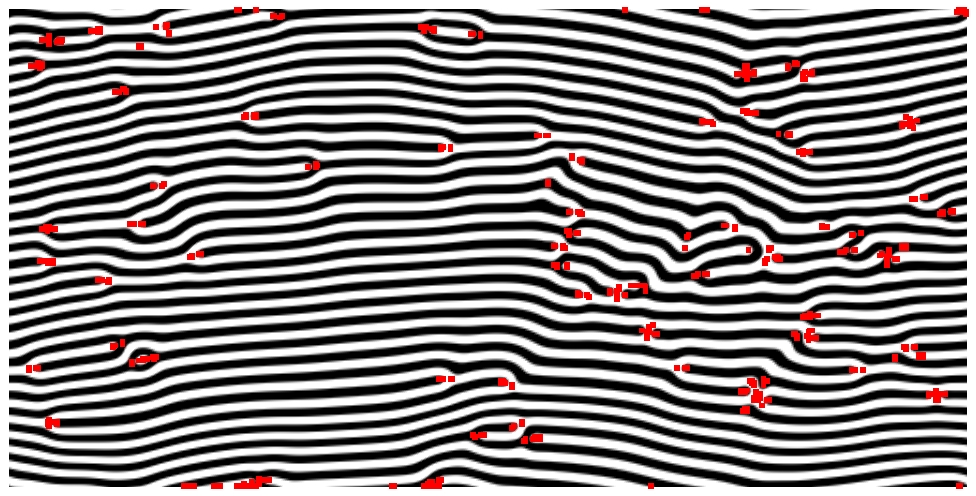
\includegraphics[angle=0,width=0.5\textwidth]{phi_defects_run774_5120.jpg}
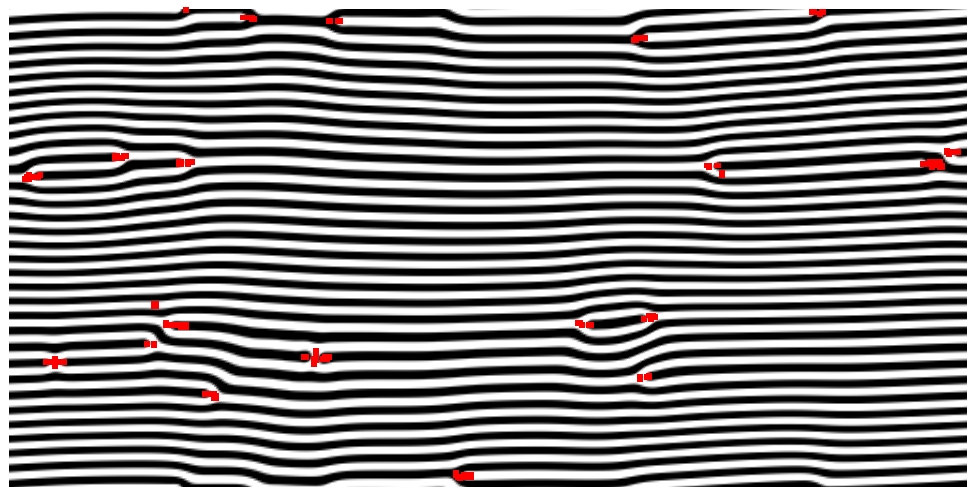
\includegraphics[angle=0,width=0.5\textwidth]{phi_defects_run774_10240.jpg}
\caption{Defect structure of system A: The pictures show results of a smaller simulation at timestep $t=5.12\e{6}$ (top) and $1.024\e{7}$ (bottom) with an imposed shear rate $\dot{\gamma}=1.25\cdot10^{-5}$. The system has been pre-sheared at various higher, subsequently lowered shear rates ranging from $\dot{\gamma}=2\e{-4}$ to the above value (see Tab.\ref{tab1}). Sites where the alignment factor $X_i$ was smaller than $0.8$ are highlighted red.}
\label{fig5}
\end{figure}
This degree of defect annihilation is only found below a critical shear rate where defects are advected smoothly on well aligned lamellae, approach each other and cancel.
Above the critical shear rate the lamellae buckle quite similar to what has been reported in \cite{Gonnella98}, the structure shows a tendency to trip over itself which creates new defects.
The critical value is different in both systems, roughly between $\dot{\gamma}=2.5-5\e{-5}$ in the stiffer system A and higher at around $\dot{\gamma}=1-2\e{-4}$ in the softer system B.
Fig. \ref{fig6} shows the  complete time evolution of the defects density $\rho_D$ of system A for a sequence of decreasing shear rates.
The runs with the two highest shear rates were started from the quiescent equilibrated state, whereas all others used the final configuration of the preceding run with higher shear rate as initial configuration.
Here and in the following figures horizontal lines are time averages for the particular quantities where we think the system has reached a steady state. 
The total strain between the beginning and end of every individual run was at least $10^{5}\%$.
Interestingly once the shear rate has been decreased to the next lower rate, both systems A and B show an trend to anneal defects instantaneously or after a short latency time if the shear rate is rather low.
If the shear rate is turned up again, the lamellae buckle and the structure begins to trip over itself, once again creating new defects.
\begin{figure}[!]
\centering
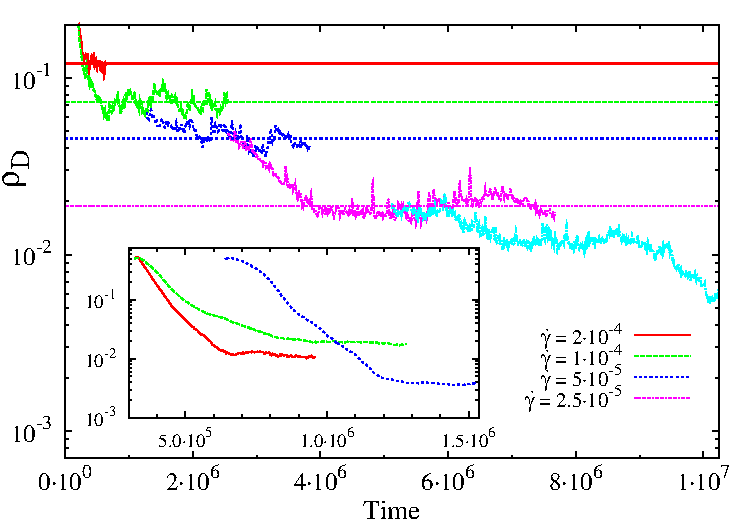
\includegraphics[angle=0,width=0.5\textwidth]{defect_density_5e-4.pdf}
\caption{Defect density $\rho_D$ vs time: The main picture shows data for system A of a sequence of simulations with consecutively lowered shear rate $\dot{\gamma}=2\e{-4}$ (red solid), $1\e{-4}$ (green long-dashed),  $5\e{-5}$ (blue short-dashed),  $2.5\e{-5}$ (magenta dotted) and  $1.25\e{-5}$ (cyan dashed-dotted). Horizontal lines indicate averages over time for the particular quantities, where we assume the system has reached a steady state. The inset gives data for the 3D-system C and shear rates $\dot{\gamma}=2\cdot10^{-4}, 1\cdot10^{-4}$ and $5\cdot10^{-5}$.} 
\label{fig6}
\end{figure}
This suggests that there is a dynamical equilibrium between defect creation and annihilation above a critical shear rate, while below the critical value defects get not anymore widely generated and the system anneals its defects and forms properly aligned lamellae.
In order to test this assumption we performed simulations starting from a very well aligned state and increased the shear rate.
The defect density goes indeed up (not shown) and reaches similar values to those shown in Fig. \ref{fig6}.
However it takes some time before a steady state is reached as the applied shear rates are rather low.\\
Fig \ref{fig7} shows the average total shear stress density $\langle \sigma_{xy}\rangle$, i.e. the total shear stress per unit lattice volume.
In the following we will drop the backets $\langle\dots\rangle$ for simplicity and write $\langle \sigma_{xy}\rangle\equiv  \sigma_{xy}$.
While for the highest applied shear rate the hydrodynamic part forms the largest contribution to the total stress density, a regime where the chemical stress dominates is entered on decreasing the shear rate.
At low shear rates stress fluctuations become more stretched in time and get smaller, what is slightly hidden by the logarithmic scale of Fig. \ref{fig7}
Their magnitude is about three times smaller in the larger simulation shown in Fig. \ref{fig1}, \ref{fig2}.
Fortunately we found that the average shear stress density over time is to a good degree independent of the system size and therefore it is justified to simulate longer times by using a smaller system size without flawing the results.
\begin{figure}[!]
\centering
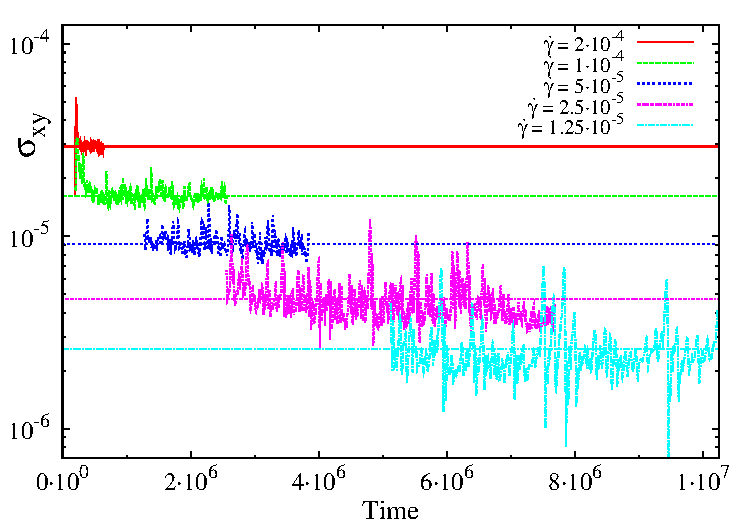
\includegraphics[angle=0,width=0.5\textwidth]{S_xy_tot_t_5e-4.pdf}
\caption{Average total shear stress $\sigma_{xy}$ versus time for system A: The horizontal lines are steady state time averages}
\label{fig7}
\end{figure}
Furthermore the stress fluctuations represent a physical aspect as they can be related to the inhomogeneities of the order parameter.
System A shows clear shear thinning behaviour and seems to obey a power law (see Fig. \ref{fig11}).
For shear rate $\dot{\gamma}=1.25\e{-5}, 2.5\e{-5}, 5\e{-5}, 1\e{-4}, 2\e{-4}$ the time averaged apparent viscosities are $\eta_{app}=\sigma_{xy}/ \eta \dot{\gamma}=2.49, 2.25, 2.18, 1.93, 1.74$.
Stress fluctuations cause temporary variations of these mean values of up to a factor 3 at the lowest shear rate.
In contrast to system A system B does not exhibit a clear monotonous shear thinning tendency.
The apparent viscosities are $\eta_{app}=1.57, 1.62, 1.55, 1.42, 1.87$ for the above shear rates and follow more a horizontal trend when the shear rate is decreased.
The stress fluctuations and time averaged shear stress densities are slightly smaller than in the stiffer system A with one exception.
For the highest shear rate $\gd=2\e{-4}$ the shear stress turns out to be larger than in system A.\\
The deviatoric part of the average chemical pressure density $\langle P_{xy}\rangle\equiv P_{xy}$ for system A is shown in the main picture of Fig. \ref{fig8}.
The fluctuations are in phase with those of the total stress in Fig. \ref{fig7} and decrease with decreasing shear rate.
System B shows a very steep decrease of $P_{xy}$ during the simulation with $\gd=1\e{-4}$, which is because of the defect annihilation.\\
\begin{figure}[!]
\centering
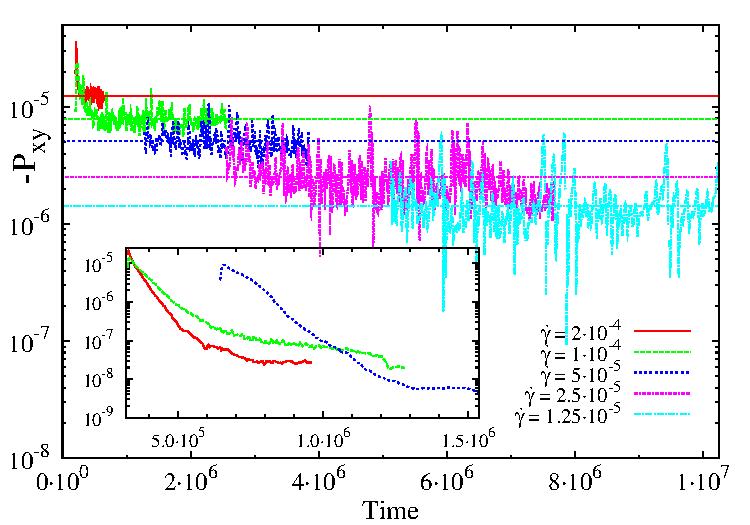
\includegraphics[angle=0,width=0.5\textwidth]{P_xy_chem_t_5e-4.pdf}
\caption{Average chemical contribution to the pressure tensor $\langle P_{xy}^{chem}\rangle$ vs time for system A. The inset shows data for the 3D-system (system C) and shear rates $\dot{\gamma}=2\cdot10^{-4}, 1\cdot10^{-4}$ and $5\cdot10^{-5}$.}
\label{fig8}
\end{figure}
Fig. \ref{fig9} illustrates the relation between $P_{xy}$ and the defect density $\rho_D$.
The black line represents a fit to the system A, which shows a linear dependence almost down to the lowest shear rate.
The result for the softer system B is slightly more obscured as a consequence of the ordering and the tendency to anneal defects.
Our quantifying protocol is based on averaging over a larger number of defects sites and is prone to inaccuracy in a regime where defects are rather scarce.
\begin{figure}[!]
\centering
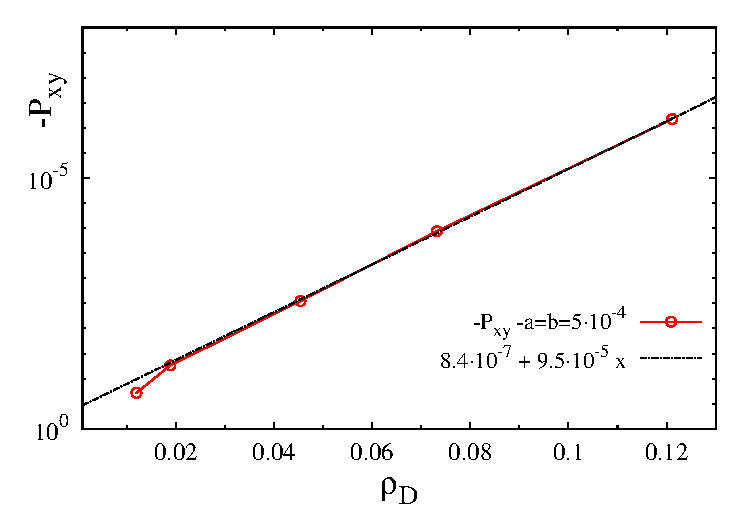
\includegraphics[angle=0,width=0.5\textwidth]{P_xy_defect_density.pdf}
\caption{Average chemical contribution to the pressure tensor $\langle P_{xy}^{chem}\rangle$ vs defect density for system A ($\eta=8.33\cdot10^{-2}, -a=b=5\cdot 10^{-4}$)} 
\label{fig9}
\end{figure}
The main picture in Fig. \ref{fig10} shows averaged first normal stress differences $\langle N_1\rangle \equiv N_1$ versus time for system A.
At first until $\gd=5\e{-5}$ the first normal stress differences decrease monotonously with decreasing shear rate.
At lower shear rates, however, the behaviour is far from being monotonous and $N_1$ rises again.
This makes it difficult or even impossible to define reasonable time averages as $N_1$ may still evolve at the end of the run.
\begin{figure}[!]
\centering
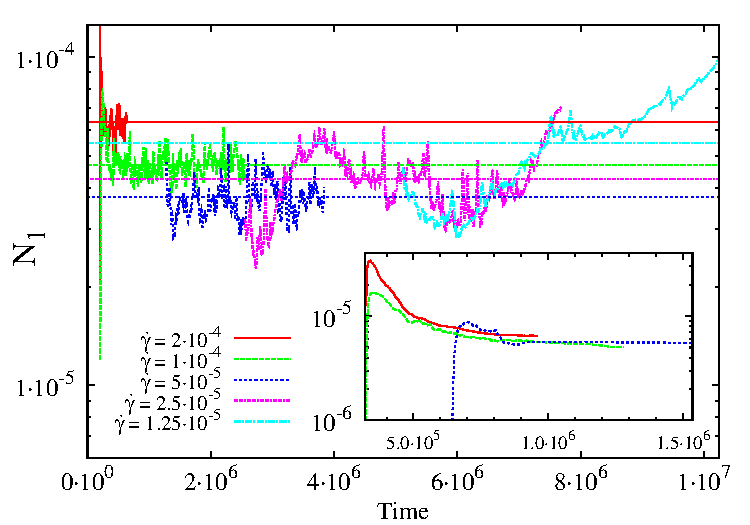
\includegraphics[angle=0,width=0.5\textwidth]{N1_t_5e-4.pdf}
\caption{Average first normal stress differences $\langle N_1 \rangle= \langle \sigma_{xx}-\sigma_{yy}\rangle$ vs time for system A1. The inset shows data for the 3D-system (system C) and shear rates $\dot{\gamma}=2\cdot10^{-4}, 1\cdot10^{-4}$ and $5\cdot10^{-5}$.}
\label{fig10}
\end{figure}
This feature is actually less erratic than it seems at first sight and can be rationalised. 
A look at Fig. \ref{fig6} reveals that $N_1$ rises in the same way as the defect density drops.
A pair of defects can cancel if one of them is an endpoint of a black lamella surrounded by a branching white lamella and the other one is a white endpoint surrounded by a branching black lamella.
When these two defects anneal the lamella spacing increases locally by half a lamellar width.
The interfaces have to expand in y-direction as the system is not frustrated enough to create an entire new layer in order to get the lamellar width back closer to its equilibrium value.
Hence the normal stresses $\sigma_{yy}$ become negative and consecutively smaller, leading to gradually larger values of $N_1$.
It should be stressed that only $\sigma_{yy}$ seems to evolve anomalously slowly and all other components of the stress tensor reach state state values more rapidly.
System B again behaves different in the sense that $N_1$ continues to fall for lower shear rates despite there is also ongoing annealing of defects.
This difference is a direct effect of the softness of system B, whose smaller Landau coefficients prevent the normal stresses $\sigma_{yy}$ from taking up very negative values and $N_1$ from rising.
Nevertheless close to the end of the simulations with the two lowest shear rates $N_1$ is still slightly changing which suggests that this slowly evolving behaviour is also due to ongoing defect annihilation.
Because both trends in system A and B are consequences of the impossibility to optimize the lamellar width, larger simulations should lead to more defined steady state values for $N_1$.
However, we were not able to check this as this proves computationally cosly.\\
In Fig. \ref{fig11} we show flowcurves derived from time averages of $\sigma_xy$ and $N_1$ as a function of shear rate.
The time average of shear stress density in systems A follow a power law $\sigma_{xy}=\dot{\gamma}^m$ with an exponent $m\simeq 0.87$ and gives evidence for shear thinning behaviour.
In case of system B the best fit for the lowest three shear rate is obtained for an exponent $m=1$, indicationg more or less constant viscosity and no shear thinning.
It is not very surprising as the chemical contribution to the total stress almost vanishes for shear rates $\dot{\gamma}\le1\e{-4}$ due to the significant decrease of the number of defects.
The observed power law behaviour is simply that of the hydrodynamic part of the stress, which is linear in our case.\\
A comparison with experimental work remains difficult because the topology of defects differ in two and three dimensions.
\begin{figure}[!]
\centering
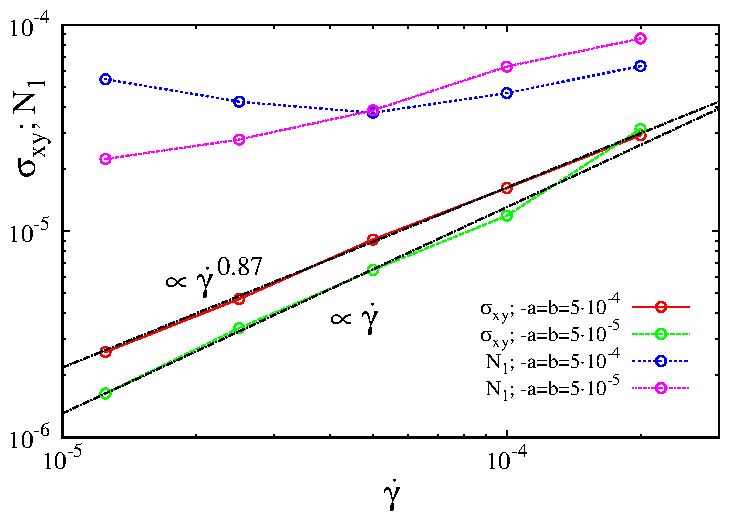
\includegraphics[angle=0,width=0.5\textwidth]{S_xy_N1_gammadot.pdf}
\caption{Flowcurves: Average shear stress $\langle \sigma_{xy}\rangle$ and first normal stress differences $\langle N_1 \rangle$ vs shear rate $\dot{\gamma}$ for system A ($\eta=8.33\cdot10^{-2}, -a=b=5\cdot 10^{-4}$)} 
\label{fig11}
\end{figure}
Our two-dimensional system is translational invariant in the third dimension.
So every branch point or endpoint of a lamella has the topology of an edge defect in the 3D-counterpart of the structure.
Moreover screw defects do not exist in our picture as they can only occur in more than two dimensions.
A recent experimental and theoretical work studies the nonlinear relation between shear stress and shear rate in lyotropic lamellar phases \cite{Lu08}
Interestingly the authors identify exactly the motion of screw defects as the key mechanism responsible for the layer tilting and defect formation. 
For the power law dependence of the shear stress on the shear rate they find an experimental value of $m\simeq=1/1.44\simeq 0.694$, which is in good agreement with their theoretical prediction of $m=2/3$.\\
Contrary to shear stresses first normal stress differences do not level off because of ongoing defect annihilation.
Neither system A nor B is in a steady state at the end of the simulation and therefore the data for $N_1$ is only shown for the sake of completeness.



\subsection*{Results in Three Dimensions}

The computational costs of a detailed analysis of the nonlinear rheology in three dimensions are still substantial as for steady state quantities it is necessary to simulate large strains.
Therefore we performed only a limited number of simulations for selected parameters. 
\begin{figure}[!]
\centering
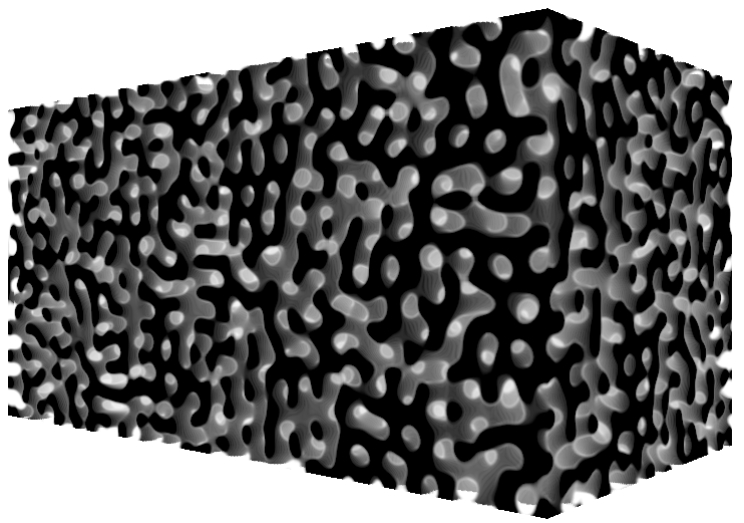
\includegraphics[angle=0,width=0.45\textwidth]{phi_run786_320.jpg}
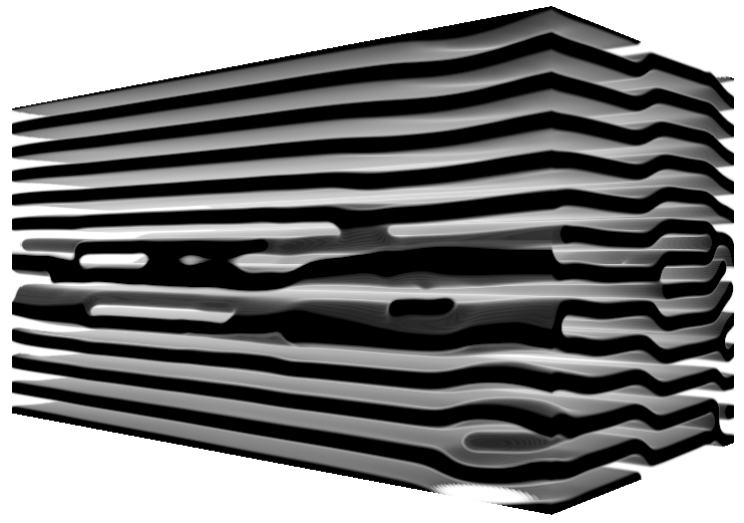
\includegraphics[angle=0,width=0.45\textwidth]{phi_run788_960.jpg}
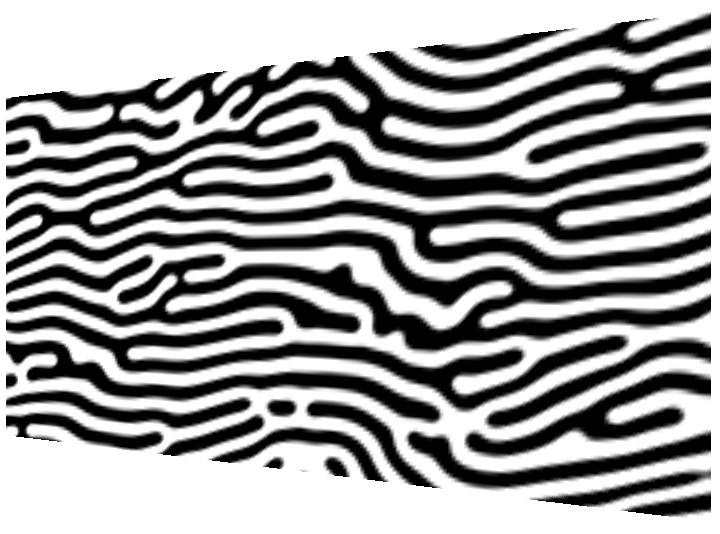
\includegraphics[angle=0,width=0.45\textwidth]{phi_run792_960.jpg}
\caption{Order parameter $\phi$ in two and three dimensions: The top and centre picture show system C after equilibration at timestep $t=3.2\e{5}$ and in shear flow ($\dot{\gamma}=1\cdot10^{-4}$) at $t=9.6\e{5}$, where shear-induced layering takes place. The image at the bottom depicts the corresponding two dimensional system A of the same size in flow and velocity gradient direction.} 
\label{fig12}
\end{figure}
For our three dimensional simulations, in the following referred to as system C, we used parameters identical to those of the stiffer 2D-system A, but reduced the system size to $N_x\times N_y \times N_z=128\times256\times128$ lattice sites.
The directions of vorticity, flow and velocity gradient are now x, y and z, respectively.\\ 
The top picture in Fig. \ref{fig12} shows the order parameter $\phi$ after equilibration at time step $t=3.2\e{5}$ prior to shearing, which served as initial configuration for the runs with shear rate $\gd=1\e{-4}$ and $2\e{-4}$.
A corresponding configuration, which was equilibrated for another $3.2\e{5}$ timesteps was used for the run with $\gd=\e{-5}$.
As before black and white correspond to $\phi=-1$ and $\phi=1$, repectively, whereas gray scales give intermediate values of $\phi$.
The opacity of $phi$ has been linearly reduced from its full value at $\phi=-1$ to 0 at $\phi=1$ in order to reveal the lamellar structure close to the  boundaries.
In comparison to the 2D-case the isosurfaces of the cuboid, taken as quasi-two-dimensional equivalent in 3D, exhibit a slightly different morphology with shorter protrusions and an overall pattern, which appears somewhat more irregular.
Nonetheless the quiescent and equilibrated system C adopts the same lamellar spacing of about 10 lattice sites as system A.Fig. \ref{fig13} shows a slice through $C({\bm k})$ along $k_y=0$ (cuts along $k_x,k_z=0$ look identical), which resembles the left picture in Fig. \ref{fig4} and differs only in the magniude.\\ 
However, in shear flow system A and C behave very differently.
Even for the highest shear rate we applied and contrary to the 2D-case system C orders readily into a regular lamellar structure.
The centre picture of Fig.\ref{fig12} shows an example at timestep $t=9.6\e{5}$ and shear rate $\gd=1\e{-4}$, which we picked as this was the least ordered one of all three runs.
With a total number of 13 layers the lamellar spacing is still close to the equilibrium value of roughly 10 lattice sites.
Besides some irregularities at the front boundary there are obviously edge defects, caused by a branching of the lamellae and visible at the very top and bottom in the foreground and more towards the centre in the background.
\begin{figure}[!]
\centering
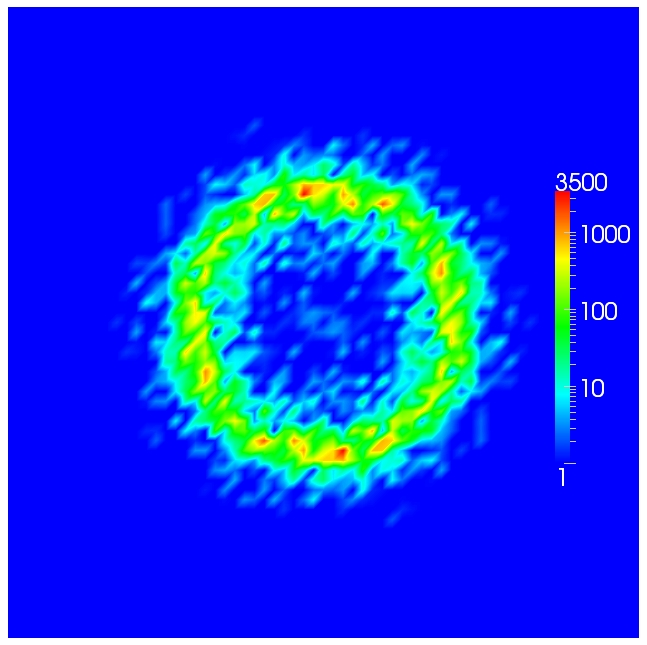
\includegraphics[angle=0,width=0.35\textwidth]{ck_y-slice_run786_320.jpg}
\caption{Structure factor $C({\mathbf k})$ of quiescent system C, showing a cut along $k_y=0$ after equilibration at $t=3.2\e{5}$. Shown are wavevectors on the interval $k_x, k_z\in[-\pi/2 l,\pi/2 l]$.}
\label{fig13}
\end{figure}
\begin{figure*}[!]
\centering
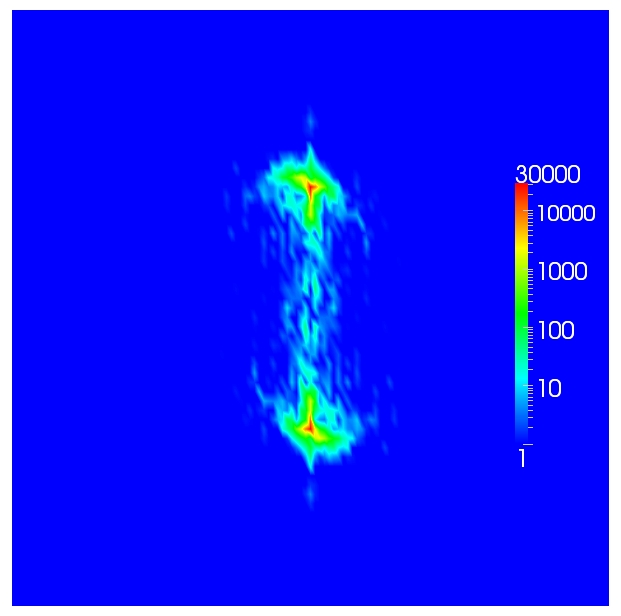
\includegraphics[angle=0,width=0.33\textwidth]{ck_x-slice_run788_960.jpg}
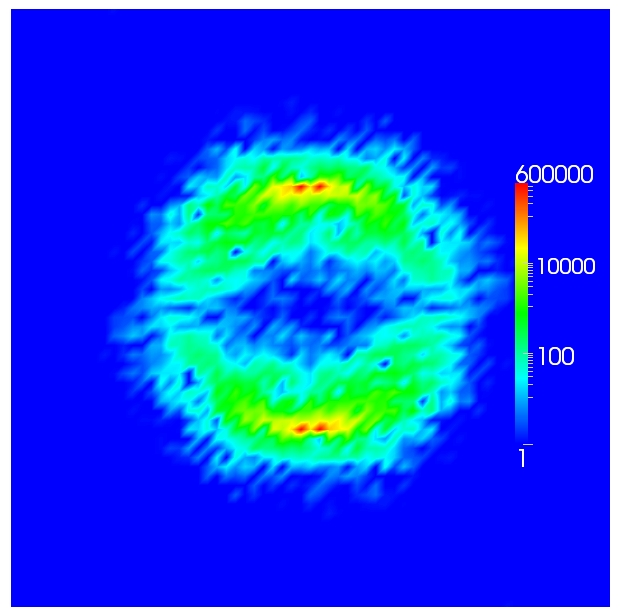
\includegraphics[angle=0,width=0.33\textwidth]{ck_y-slice_run788_960.jpg}
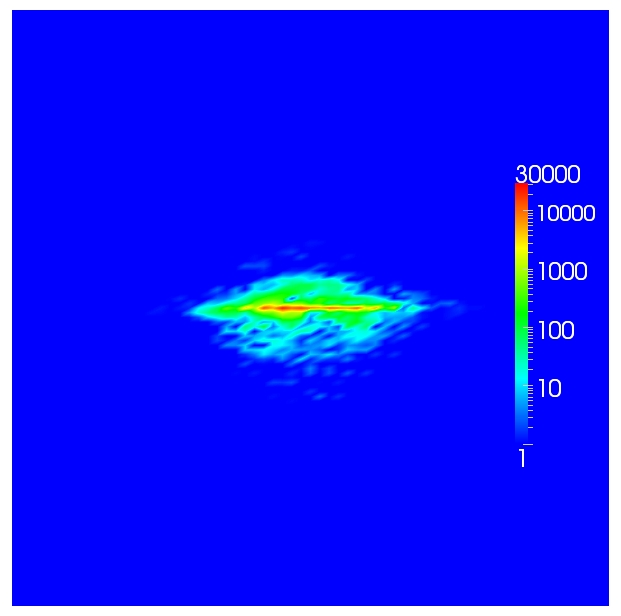
\includegraphics[angle=0,width=0.33\textwidth]{ck_z-slice_run788_960.jpg}
\caption{Structure factor $C({\mathbf k})$ of system C in shear flow ($\dot{\gamma}=1\cdot10^{-4}$) at t=960k: Cuts through along $k_x=0,k_y=0$ and $k_z=3\pi/16 l$, respectively are shown for wavevectors $k_x, k_y, k_z\in[-\pi/2 l,\pi/2 l]$. Note that in these images y is the flow direction, whereas the direction of the velocity gradient and vorticity are z and x, respectively.}
\label{fig14}
\end{figure*}
The edge defects emerge from the spontaneous shear-induced ordering of the phase separated structure but remain very localised at first.
As a result of shear advection the interfaces spread and close gaps at later times to finally form either continuous lamellae or uniform edges, which are oriented along the flow, virtually stable and do not anneal.
The fact that separated regions with similar order parameter values can now also connect along a third direction and expell regions with opposite order parameter, seems to play a key role pertaining to the formation of a homogenously layered structure.
The bottom picture in Fig. \ref{fig12} gives an idea about how the dimesionality affects the morphology of layered smectics and binary fluids.
It shows the two-dimensional system A as slice of system C along the direction of vorticity.
The difference between both systems is striking and even more surprising as both results were obtained with the same parameter setting and identical equilibration and shear histories.
The inset of Fig. \ref{fig6} quantifies the time it takes system C to order into a layererd defect-scarce structure.
Within a few $10^5$ timesteps the defect density of system C decreases to magnitudes, which we obtained in the 2D-case only for shear rates about one decade lower and times about a factor 10 longer.\\
Scarce defects lead to smaller chemical pressure, which is shown in the insets of Fig. \ref{fig8} for the component $P_{xy}$.
The hydrodynamic part of the stress is by far dominating and shear thinning occurs to an ultimate degree where the apparent viscosity of the fluid is that of the solvent and the chemical contribution has practically vanished.
A relation between the deviatoric chemical pressure tensor and the defect density like in Fig. \ref{fig9} can therefore not be established.
The inset of Fig.\ref{fig10} shows first normal stress differences $N_1=\langle\sigma_{yy}-\sigma{zz}\rangle$.
For all shear rates $\gd5\e{-5}-2\e{-4}$ system C takes similar values, which are monotonously approached and about one decade smaller than those for $N_1$ of system A.\\ 
Finally we want to glimpse at the structure factor of system C in shear flow.
Fig. \ref{fig14} shows $C({\bm k})$ at shear rate $\gd=1\e{-4}$ for Fourier vectors on the interval $[-\pi/2 l, \pi/ 2 l]$.
The leftmost picture is a cut along $k_x=0$ in with $k_y$ in horizontal and $k_z$ in vertical direction.
It shows data in flow-velocity-gradient plane and compares directly with the left picture in Fig. \ref{fig4}.
The pictures in the centre and on the right give cuts along $k_y=0$ in $k_x-k_z$-plane and along $k_z$ in $k_x-k_y$-plane. 
Note the scale of the logarithmic color map in the centre picture.
Despite a certain similarity with the 2D-structure after switch off in the rightmost picture of Fig. \ref{fig4}, the structure factor in three dimensions has a very pronounced peak at $k_z\simeq\pm0.2\pi/l$.
It appears to be split into two parts, but this is an effect of the relatively sparse discretization and caused by the visualization software.
Although strongly preaked, the spatial dependence of the signal is best demonstrated in a 3D-representation. 
Fig. \ref{fig15} depicts the structure factor in 3D, whereas the red area corresponds to an isosurface of about $C({\bm k})\simeq 10^3$.
It reveals a banana-shaped spatial dependence with some small appendices in flow direction at $k_x=0$.

\begin{figure}[!]
\centering
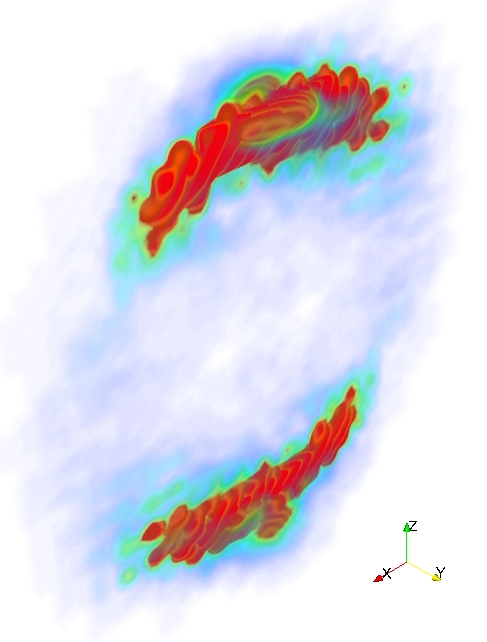
\includegraphics[angle=0,width=0.45\textwidth]{ck_run788_960_zoom.jpg}
\caption{Structure factor $C({\mathbf k})$ of system C in shear flow: The picture gives a 3D-representation of the data in shear flow at $t=9.6\e{5}$ and $\dot{\gamma}=1\cdot10^{-4}$.}
\label{fig15}
\end{figure}

\begin{table}[htp]
\small
\caption{Simulation parameters: The systems were first equilibrated from spinodal decomposition at zero shear rate (EQ), followed by various shear rates, ranging from $\dot{\gamma}=2\cdot10^{-4}$ till $1.25\cdot10^{-5}$. For some runs a final switch off (SO) at zero shear rate was performed. The parameters $\kappa=-6\cdot10^{-4}, c=7.6\cdot10^{-4}, M=0.25$ and $\eta=8.33\cdot10^{-2}$ were the same throughout all simulations.}
  \label{tab1}
%  \begin{tabular*}{0.48\textwidth}{@{\extracolsep{\fill}}lllll}
  \begin{tabular*}{0.495\textwidth}{lllll}
\hline
run \# & $N_x\times N_y\times N_z$ & time $\cdot 10^3$ & -a=b &  $\dot\gamma$\\
\hline
system A & & & &\\
\hline 
703 & $1024\times512\times1$ & 0-320 & $5\cdot10^{-4}$ & 0 - EQ  \\
704 & $1024\times512\times1$ & 320-640& $5\cdot10^{-4}$ & $1\cdot10^{-4}$\\
705 & $1024\times512\times1$ & 640-960& $5\cdot10^{-4}$ & 0 - SO-4 \\
\hline
767 & $512\times256\times1$ & 0-320 & $5\cdot10^{-4}$  & 0 - EQ\\
775 & $512\times256\times1$ & 320-640& $5\cdot10^{-4}$ & $2\cdot 10^{-4}$ \\
769 & $512\times256\times1$ & 320-2560& $5\cdot10^{-4}$ & $1\cdot 10^{-4}$ \\
771 & $512\times256\times1$ & 1280-3840& $5\cdot10^{-4}$ & $ 5\cdot10^{-5}$ \\
772 & $512\times256\times1$ & 5120-7680& $5\cdot10^{-4}$ & $ 2.5\cdot10^{-5}$ \\
774 & $512\times256\times1$ & 5120-10240& $5\cdot10^{-4}$ & $1.25\cdot10^{-5}$ \\
\hline
792 & $256\times128\times1$ & 320-1600& $5\cdot10^{-4}$ & $1\cdot10^{-4}$ \\
system B & & & &\\
\hline
707 & $1024\times512\times1$ & 0-320 & $5\cdot10^{-5}$ & 0 - EQ \\
710 & $1024\times512\times1$ & 320-960& $5\cdot10^{-5}$ & $1\cdot10^{-4}$ \\
765 & $1024\times512\times1$ & 960-1280& $5\cdot10^{-5}$ & 0 - SO-4 \\
\hline
776 & $512\times256\times1$ & 0-320 & $5\cdot10^{-5}$ & 0 - EQ\\
777 & $512\times256\times1$ & 320-960& $5\cdot10^{-5}$ & $2\cdot 10^{-4}$ \\
778 & $512\times256\times1$ & 320-2560& $5\cdot10^{-5}$ & $1\cdot 10^{-4}$ \\
780 & $512\times256\times1$ & 1280-3840& $5\cdot10^{-5}$ & $5\cdot 10^{-5}$ \\
781 & $512\times256\times1$ & 2560-6400& $5\cdot10^{-5}$ & $2.5\cdot 10^{-5}$ \\
782 & $512\times256\times1$ & 5120-7680& $5\cdot10^{-5}$ & $1.25\cdot 10^{-5}$ \\
\hline
system C & & & &\\
\hline
786 & $128\times256\times128$ & 0-640 & $5\cdot10^{-4}$ & 0 - EQ\\
787 & $128\times256\times128$ & 320-640 & $5\cdot10^{-4}$ & $2\cdot 10^{-4}$\\
788 & $128\times256\times128$ & 320-960 & $5\cdot10^{-4}$ & $1\cdot 10^{-4}$\\
789 & $128\times256\times128$ & 640-1280 & $5\cdot10^{-4}$ & $5\cdot 10^{-5}$\\
\hline
\end{tabular*}
\end{table}

\section{Conclusions}
We have performed large scale simulations of a lamellar system in steady shear flow  in two and three dimensions.
We were able to relate the morphology of the order parameter in the quiescent state to results from previous studies of the same system using similar parameters.\\
In two dimensions and steady state simple shear flow at Peclet numbers ${\cal O}(10)$ we did not observe a homogenous lamellar structure for shear rates above a critical threshold, which depends on the exact parametrization of the free energy functional.
The morphology was rather inhomogenous instead, exhibiting regions that are under pressure with lamellar spacings smaller than the equilibrium value and others that were stretched.
We could relate the structure to typical values of rheological quantities.
Areas under extensional flow coincide with locally negative or small positive shear stresses and first normal stress differences, whereas both go to positive peak values in the compressed domains.
Below a critical shear rate the systems showed no tendency anymore to trip over itself and defects annealed as they could approach each other in adjacent lamellae.
The characteritic time of this process was set by the shear rate and the total strain.
The deviatoric part of the chemical pressure was correlated to the number of defect sites, wheras the latter was measured by means of an alignment factor, which quantified the localby curvature of the lamellar interfaces.
For the stiffer system A we could verify a linear relation between the defect density and the average chemical contribution to the shear stress.\\ 
In system A first normal stress differences decreased as long as a dynamic equilibrium between defect creation an annihilation existed.
Below the critical threshold this was no longer the case and pronounced defect annealing caused a rise in the first normal stress differences as the average lamellar spacing increased.
We could establish a shear thinning regime for the more defect ladden system A.
System B in contrary was so perfectly annealed in the steady state that virtually shear stresses were down at the hydrodynamic level and the relation between shear stress and shear rate was trivially linear.\\
In three dimensions we simulated shear strains which have not been attained so far.
Interestingly for the same parameters we observe striking differences between system A in 2D and system C in 3D.
It seems that the dynamics of the defects in two and three dimensions is rather incommensurable.
Even at the lowest applied shear rates the chemical stress has decayed to a level where the apparent viscosity was virtually identical to the solvent.
Structure factor data confirmed the very regular layered ordering of the structure and a lamellar spacing close to the equilibrium value. 


\section{Acknowledgements}


\footnotesize{
\bibliography{smectics} %your .bib file
\bibliographystyle{rsc} %the RSC's .bst file
}

\end{document}
